% Options for packages loaded elsewhere
\PassOptionsToPackage{unicode}{hyperref}
\PassOptionsToPackage{hyphens}{url}
%
\documentclass[
]{article}
\usepackage{amsmath,amssymb}
\usepackage{lmodern}
\usepackage{iftex}
\ifPDFTeX
  \usepackage[T1]{fontenc}
  \usepackage[utf8]{inputenc}
  \usepackage{textcomp} % provide euro and other symbols
\else % if luatex or xetex
  \usepackage{unicode-math}
  \defaultfontfeatures{Scale=MatchLowercase}
  \defaultfontfeatures[\rmfamily]{Ligatures=TeX,Scale=1}
\fi
% Use upquote if available, for straight quotes in verbatim environments
\IfFileExists{upquote.sty}{\usepackage{upquote}}{}
\IfFileExists{microtype.sty}{% use microtype if available
  \usepackage[]{microtype}
  \UseMicrotypeSet[protrusion]{basicmath} % disable protrusion for tt fonts
}{}
\makeatletter
\@ifundefined{KOMAClassName}{% if non-KOMA class
  \IfFileExists{parskip.sty}{%
    \usepackage{parskip}
  }{% else
    \setlength{\parindent}{0pt}
    \setlength{\parskip}{6pt plus 2pt minus 1pt}}
}{% if KOMA class
  \KOMAoptions{parskip=half}}
\makeatother
\usepackage{xcolor}
\usepackage[margin=1in]{geometry}
\usepackage{color}
\usepackage{fancyvrb}
\newcommand{\VerbBar}{|}
\newcommand{\VERB}{\Verb[commandchars=\\\{\}]}
\DefineVerbatimEnvironment{Highlighting}{Verbatim}{commandchars=\\\{\}}
% Add ',fontsize=\small' for more characters per line
\usepackage{framed}
\definecolor{shadecolor}{RGB}{248,248,248}
\newenvironment{Shaded}{\begin{snugshade}}{\end{snugshade}}
\newcommand{\AlertTok}[1]{\textcolor[rgb]{0.94,0.16,0.16}{#1}}
\newcommand{\AnnotationTok}[1]{\textcolor[rgb]{0.56,0.35,0.01}{\textbf{\textit{#1}}}}
\newcommand{\AttributeTok}[1]{\textcolor[rgb]{0.77,0.63,0.00}{#1}}
\newcommand{\BaseNTok}[1]{\textcolor[rgb]{0.00,0.00,0.81}{#1}}
\newcommand{\BuiltInTok}[1]{#1}
\newcommand{\CharTok}[1]{\textcolor[rgb]{0.31,0.60,0.02}{#1}}
\newcommand{\CommentTok}[1]{\textcolor[rgb]{0.56,0.35,0.01}{\textit{#1}}}
\newcommand{\CommentVarTok}[1]{\textcolor[rgb]{0.56,0.35,0.01}{\textbf{\textit{#1}}}}
\newcommand{\ConstantTok}[1]{\textcolor[rgb]{0.00,0.00,0.00}{#1}}
\newcommand{\ControlFlowTok}[1]{\textcolor[rgb]{0.13,0.29,0.53}{\textbf{#1}}}
\newcommand{\DataTypeTok}[1]{\textcolor[rgb]{0.13,0.29,0.53}{#1}}
\newcommand{\DecValTok}[1]{\textcolor[rgb]{0.00,0.00,0.81}{#1}}
\newcommand{\DocumentationTok}[1]{\textcolor[rgb]{0.56,0.35,0.01}{\textbf{\textit{#1}}}}
\newcommand{\ErrorTok}[1]{\textcolor[rgb]{0.64,0.00,0.00}{\textbf{#1}}}
\newcommand{\ExtensionTok}[1]{#1}
\newcommand{\FloatTok}[1]{\textcolor[rgb]{0.00,0.00,0.81}{#1}}
\newcommand{\FunctionTok}[1]{\textcolor[rgb]{0.00,0.00,0.00}{#1}}
\newcommand{\ImportTok}[1]{#1}
\newcommand{\InformationTok}[1]{\textcolor[rgb]{0.56,0.35,0.01}{\textbf{\textit{#1}}}}
\newcommand{\KeywordTok}[1]{\textcolor[rgb]{0.13,0.29,0.53}{\textbf{#1}}}
\newcommand{\NormalTok}[1]{#1}
\newcommand{\OperatorTok}[1]{\textcolor[rgb]{0.81,0.36,0.00}{\textbf{#1}}}
\newcommand{\OtherTok}[1]{\textcolor[rgb]{0.56,0.35,0.01}{#1}}
\newcommand{\PreprocessorTok}[1]{\textcolor[rgb]{0.56,0.35,0.01}{\textit{#1}}}
\newcommand{\RegionMarkerTok}[1]{#1}
\newcommand{\SpecialCharTok}[1]{\textcolor[rgb]{0.00,0.00,0.00}{#1}}
\newcommand{\SpecialStringTok}[1]{\textcolor[rgb]{0.31,0.60,0.02}{#1}}
\newcommand{\StringTok}[1]{\textcolor[rgb]{0.31,0.60,0.02}{#1}}
\newcommand{\VariableTok}[1]{\textcolor[rgb]{0.00,0.00,0.00}{#1}}
\newcommand{\VerbatimStringTok}[1]{\textcolor[rgb]{0.31,0.60,0.02}{#1}}
\newcommand{\WarningTok}[1]{\textcolor[rgb]{0.56,0.35,0.01}{\textbf{\textit{#1}}}}
\usepackage{graphicx}
\makeatletter
\def\maxwidth{\ifdim\Gin@nat@width>\linewidth\linewidth\else\Gin@nat@width\fi}
\def\maxheight{\ifdim\Gin@nat@height>\textheight\textheight\else\Gin@nat@height\fi}
\makeatother
% Scale images if necessary, so that they will not overflow the page
% margins by default, and it is still possible to overwrite the defaults
% using explicit options in \includegraphics[width, height, ...]{}
\setkeys{Gin}{width=\maxwidth,height=\maxheight,keepaspectratio}
% Set default figure placement to htbp
\makeatletter
\def\fps@figure{htbp}
\makeatother
\setlength{\emergencystretch}{3em} % prevent overfull lines
\providecommand{\tightlist}{%
  \setlength{\itemsep}{0pt}\setlength{\parskip}{0pt}}
\setcounter{secnumdepth}{-\maxdimen} % remove section numbering
\ifLuaTeX
  \usepackage{selnolig}  % disable illegal ligatures
\fi
\IfFileExists{bookmark.sty}{\usepackage{bookmark}}{\usepackage{hyperref}}
\IfFileExists{xurl.sty}{\usepackage{xurl}}{} % add URL line breaks if available
\urlstyle{same} % disable monospaced font for URLs
\hypersetup{
  pdftitle={tp2},
  pdfauthor={Lapu Matthias \textbar{} Amaël Kreis},
  hidelinks,
  pdfcreator={LaTeX via pandoc}}

\title{tp2}
\author{Lapu Matthias \textbar{} Amaël Kreis}
\date{2023-02-17}

\begin{document}
\maketitle

\hypertarget{i.-variation-sous-jacente-et-uxe9chantillonnage-ruxe9puxe9tuxe9}{%
\subsection{I. Variation sous-jacente et échantillonnage
répété}\label{i.-variation-sous-jacente-et-uxe9chantillonnage-ruxe9puxe9tuxe9}}

\begin{enumerate}
\def\labelenumi{\arabic{enumi}.}
\tightlist
\item
  Si X ∼ E(0.5), quelle est la probabilité qu'on observe une valeur
  supérieure à 3?
\end{enumerate}

2.Simulez un échantillon de taille n = 20 d'un loi de E(0,5), créez un
histogramme de votre échantillon et commentez la forme de votre
histogramme. Superposer la vrai densité. Quelle est la probabilité
empirique qu'on observe une valeur supérieure à 3 ?

\begin{Shaded}
\begin{Highlighting}[]
\NormalTok{x}\OtherTok{\textless{}{-}}\FunctionTok{rexp}\NormalTok{(}\DecValTok{20}\NormalTok{,}\FloatTok{0.5}\NormalTok{)}
\FunctionTok{hist}\NormalTok{(x, }\AttributeTok{freq=}\ConstantTok{FALSE}\NormalTok{)}
\NormalTok{maxvalue }\OtherTok{\textless{}{-}} \FunctionTok{ceiling}\NormalTok{(}\FunctionTok{max}\NormalTok{(x))}
\FunctionTok{lines}\NormalTok{(}\DecValTok{0}\SpecialCharTok{:}\NormalTok{maxvalue,}\FunctionTok{dexp}\NormalTok{(}\DecValTok{0}\SpecialCharTok{:}\NormalTok{maxvalue, }\FloatTok{0.5}\NormalTok{), }\AttributeTok{col=}\StringTok{"green"}\NormalTok{,)}
\end{Highlighting}
\end{Shaded}

\includegraphics{tp2_files/figure-latex/unnamed-chunk-1-1.pdf}

Commentaire histogramme à insérer

3.Répétez cette opération 5 ou 6 fois et commentez les différences entre
les histogrammes que vous obtenez à chaque fois. Utilisez la même limite
sur les axes pour faciliter la comparaison. Notez également comment la
probabilité empirique qu'on observe une valeur supérieure à 3 change.

\begin{enumerate}
\def\labelenumi{\arabic{enumi}.}
\setcounter{enumi}{3}
\tightlist
\item
  Augmentez la taille de votre échantillon à 100 et répétez votre
  expérience. Que remarquez-vous?
\end{enumerate}

\includegraphics{tp2_files/figure-latex/unnamed-chunk-3-1.pdf}

\hypertarget{ii.-variabilituxe9-aluxe9atoire-du-maximum-de-luxe9chantillon}{%
\subsection{II. Variabilité aléatoire du maximum de
l'échantillon}\label{ii.-variabilituxe9-aluxe9atoire-du-maximum-de-luxe9chantillon}}

\hypertarget{simuler-un-uxe9chantillon-de-taille-n-10-dune-loi-u1-1-et-enregistrez-le-maximum-de-luxe9chantillon.}{%
\section{1. Simuler un échantillon de taille n = 10 d'une loi U(−1, 1)
et enregistrez le maximum de
l'échantillon.}\label{simuler-un-uxe9chantillon-de-taille-n-10-dune-loi-u1-1-et-enregistrez-le-maximum-de-luxe9chantillon.}}

\begin{Shaded}
\begin{Highlighting}[]
\NormalTok{x }\OtherTok{\textless{}{-}} \FunctionTok{runif}\NormalTok{(}\DecValTok{10}\NormalTok{, }\SpecialCharTok{{-}}\DecValTok{1}\NormalTok{, }\DecValTok{1}\NormalTok{)}
\NormalTok{max }\OtherTok{\textless{}{-}} \FunctionTok{max}\NormalTok{(x)}
\end{Highlighting}
\end{Shaded}

\hypertarget{ruxe9puxe9tez-les-deux-uxe9tapes-ci-dessus-dix-fois-en-uxe9crivant-le-maximum-de-luxe9chantillon-uxe0-chaque-fois.-commentez-la-variabilituxe9-des-valeurs-que-vous-obtenez-pour-les-maxima-de-votre-uxe9chantillon.}{%
\section{2. Répétez les deux étapes ci-dessus dix fois, en écrivant le
maximum de l'échantillon à chaque fois. Commentez la variabilité des
valeurs que vous obtenez pour les maxima de votre
échantillon.}\label{ruxe9puxe9tez-les-deux-uxe9tapes-ci-dessus-dix-fois-en-uxe9crivant-le-maximum-de-luxe9chantillon-uxe0-chaque-fois.-commentez-la-variabilituxe9-des-valeurs-que-vous-obtenez-pour-les-maxima-de-votre-uxe9chantillon.}}

\begin{Shaded}
\begin{Highlighting}[]
\ControlFlowTok{for}\NormalTok{ (i }\ControlFlowTok{in} \DecValTok{1}\SpecialCharTok{:}\DecValTok{10}\NormalTok{) \{}
\NormalTok{  x }\OtherTok{\textless{}{-}} \FunctionTok{runif}\NormalTok{(}\DecValTok{10}\NormalTok{, }\SpecialCharTok{{-}}\DecValTok{1}\NormalTok{, }\DecValTok{1}\NormalTok{)}
\NormalTok{\}}
\end{Highlighting}
\end{Shaded}

\hypertarget{ruxe9puxe9tez-100-fois-et-construisez-un-histogramme-et-une-bouxeete-uxe0-moustaches.-quelle-est-la-loi-dumaximum-m-max-1in-x-i-ouxf9-x-i-u1-1-td1-superposer-la-densituxe9-thuxe9oreique-sur-lhistogramme.-que-remarquez-vous}{%
\section{3. Répétez 100 fois et construisez un histogramme et une boîte
à moustaches. Quelle est la loi dumaximum, M = max 1≤i≤n X i où X i ∼
U(−1, 1) (TD1) ? Superposer la densité théoreique sur l'histogramme. Que
remarquez-vous
?}\label{ruxe9puxe9tez-100-fois-et-construisez-un-histogramme-et-une-bouxeete-uxe0-moustaches.-quelle-est-la-loi-dumaximum-m-max-1in-x-i-ouxf9-x-i-u1-1-td1-superposer-la-densituxe9-thuxe9oreique-sur-lhistogramme.-que-remarquez-vous}}

\begin{Shaded}
\begin{Highlighting}[]
\FunctionTok{par}\NormalTok{(}\AttributeTok{mfrow=}\FunctionTok{c}\NormalTok{(}\DecValTok{3}\NormalTok{,}\DecValTok{4}\NormalTok{))}
\ControlFlowTok{for}\NormalTok{ (i }\ControlFlowTok{in} \DecValTok{1}\SpecialCharTok{:}\DecValTok{100}\NormalTok{) \{}
\NormalTok{  x }\OtherTok{\textless{}{-}} \FunctionTok{runif}\NormalTok{(}\DecValTok{10}\NormalTok{, }\SpecialCharTok{{-}}\DecValTok{1}\NormalTok{, }\DecValTok{1}\NormalTok{)}
  \FunctionTok{hist}\NormalTok{(x)}
  \FunctionTok{boxplot}\NormalTok{(x, }\AttributeTok{horizontal =} \ConstantTok{TRUE}\NormalTok{)}
\NormalTok{\}}
\end{Highlighting}
\end{Shaded}

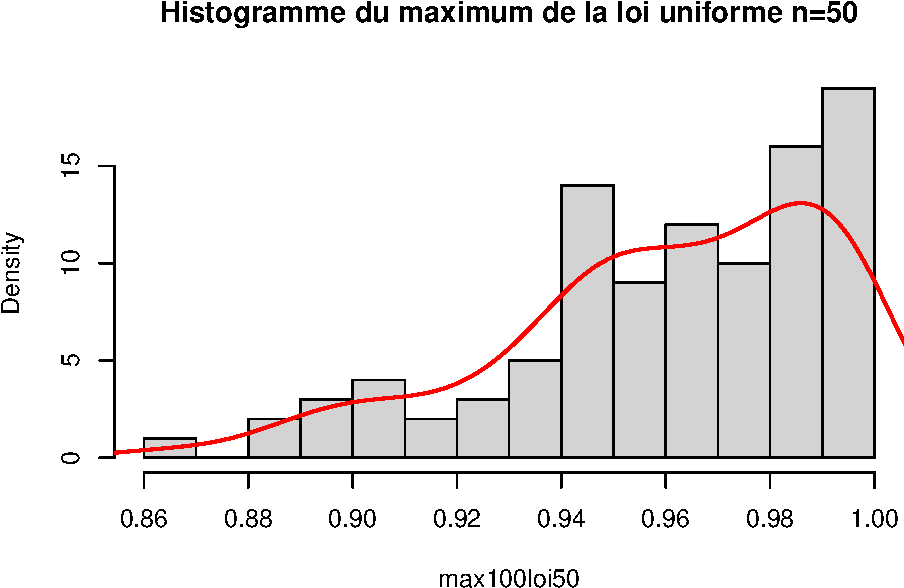
\includegraphics{tp2_files/figure-latex/unnamed-chunk-6-1.pdf}
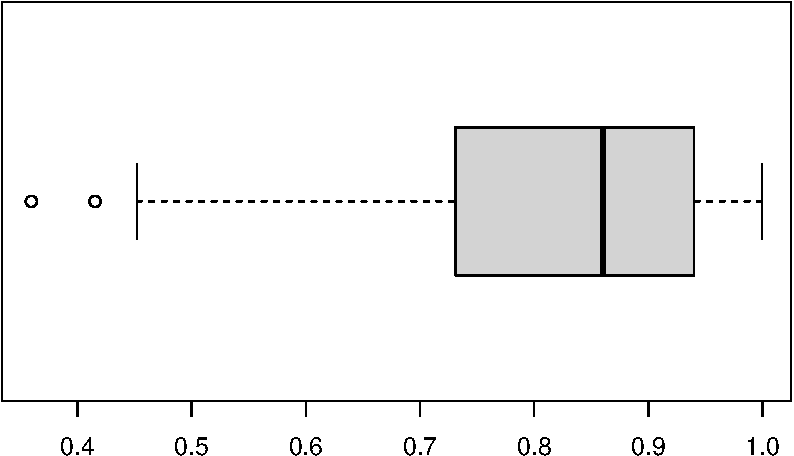
\includegraphics{tp2_files/figure-latex/unnamed-chunk-6-2.pdf}
\includegraphics{tp2_files/figure-latex/unnamed-chunk-6-3.pdf}
\includegraphics{tp2_files/figure-latex/unnamed-chunk-6-4.pdf}
\includegraphics{tp2_files/figure-latex/unnamed-chunk-6-5.pdf}
\includegraphics{tp2_files/figure-latex/unnamed-chunk-6-6.pdf}
\includegraphics{tp2_files/figure-latex/unnamed-chunk-6-7.pdf}
\includegraphics{tp2_files/figure-latex/unnamed-chunk-6-8.pdf}
\includegraphics{tp2_files/figure-latex/unnamed-chunk-6-9.pdf}
\includegraphics{tp2_files/figure-latex/unnamed-chunk-6-10.pdf}
\includegraphics{tp2_files/figure-latex/unnamed-chunk-6-11.pdf}
\includegraphics{tp2_files/figure-latex/unnamed-chunk-6-12.pdf}
\includegraphics{tp2_files/figure-latex/unnamed-chunk-6-13.pdf}
\includegraphics{tp2_files/figure-latex/unnamed-chunk-6-14.pdf}
\includegraphics{tp2_files/figure-latex/unnamed-chunk-6-15.pdf}
\includegraphics{tp2_files/figure-latex/unnamed-chunk-6-16.pdf}
\includegraphics{tp2_files/figure-latex/unnamed-chunk-6-17.pdf}

\hypertarget{augmentez-la-taille-de-votre-uxe9chantillon-uxe0-50-et-ruxe9puxe9tez-votre-expuxe9rience.-que-remarquez-vous-sont-ils-proches-de-la-symuxe9trie}{%
\section{4. Augmentez la taille de votre échantillon à 50 et répétez
votre expérience. Que remarquez-vous? Sont-ils proches de la symétrie
?}\label{augmentez-la-taille-de-votre-uxe9chantillon-uxe0-50-et-ruxe9puxe9tez-votre-expuxe9rience.-que-remarquez-vous-sont-ils-proches-de-la-symuxe9trie}}

\begin{Shaded}
\begin{Highlighting}[]
\NormalTok{x }\OtherTok{\textless{}{-}} \FunctionTok{runif}\NormalTok{(}\DecValTok{50}\NormalTok{, }\SpecialCharTok{{-}}\DecValTok{1}\NormalTok{, }\DecValTok{1}\NormalTok{)}
\end{Highlighting}
\end{Shaded}

\hypertarget{monte-carlo-methods}{%
\subsection{Monte Carlo Methods}\label{monte-carlo-methods}}

\hypertarget{moyenne-et-phuxe9nomuxe8ne-de-concentration.}{%
\section{Moyenne et phénomène de
concentration.}\label{moyenne-et-phuxe9nomuxe8ne-de-concentration.}}

\begin{enumerate}
\def\labelenumi{\arabic{enumi}.}
\tightlist
\item
  Supposons que la variance σ2 = V {[}ψ(X){]} \textless{} ∞. Donner une
  borne de cette quantité en utilisant l'inégalité de Bienaymé
  Chebychev.
\end{enumerate}

On trouve grace à l'inégalité de Bienaymé Chebychev:

\$\$

a\^{}\{2\}P(\textbar{}\psi(X) - \theta\textbar{} \ge a)
\le V{[}\psi(X){]}

\$\$

2. En supposant que a ≤ ψ(Xi) ≤ b, donner une borne en utilisant
l'inégalité de Hoeffding.

Posons : \[
S_{n} = \sum_{k=1}^n \psi(X_k)
\] D'après l'énoncé, nous savons que : \[
\frac{1}{n} \sum_{i=1}^n \psi(X_i) = \hat{\theta}
\] Ainsi : \[
\frac{S_n}{n} = \hat{\theta} 
\] Donc : \[
S_n=n\hat{\theta}
\]

D'après l'inégalité de Hoeffding nous savons que : \[
P(|S_n - E(S_n)| \geq t) \leq 2exp(\frac{-2t²}{\sum_{k=1}^n (b_k-a_k)²})
\]

Calculons l'esperance de S\_n: \[
E(S_n) = E(\sum_{k=1}^n \psi(X_k)) = \sum_{k=1}^n E(\psi(X_k)) = \sum_{k=1}^n \theta = n\theta
\] Ainsi : \[
P(|n\hat{\theta} - n\theta| \geq t) \leq 2exp(\frac{-2t²}{\sum_{k=1}^n (b_k-a_k)²})
\\
P(|\hat{\theta} - \theta| \geq \frac{t}{n}) \leq 2exp(\frac{-2t²}{\sum_{k=1}^n (b_k-a_k)²})
\] On pose : \[
\frac{t}{n} = \delta
\\
P(|\hat{\theta} - \theta| \geq \delta) \leq 2exp(\frac{-(2n\delta)²}{\sum_{k=1}^n (b_k-a_k)²})
\]

\hypertarget{thuxe9oruxe8me-central-limite-et-estimation-monte-carlo}{%
\subsection{Théorème Central Limite et Estimation Monte
Carlo}\label{thuxe9oruxe8me-central-limite-et-estimation-monte-carlo}}

1. Vérifier que l'espérance théorique d'une loi de Pareto est E {[}X{]}
= αa/α−1.

\[
P(X\le t)= (1-\left( \frac{a}{t} \right)^{\alpha}) , \;avec \;x \ge a
\]

Donc :

\$\$

E(X) = \int\_0\^{}\{+\infty\} 1-P(X \le t)dt \textbackslash{} =
\int\_0\^{}\infty  \textbackslash{} =
a+a\^{}\{\alpha\}\int\_a\^{}\{+\infty\}\frac{1}{t^{\alpha}}dt=a +
\frac{a}{\alpha -1} =\frac{\alpha a}{\alpha -1} \$\$

2. Simuler N = 1000 échantillons i.i.d de loi commune Pareto P(a, α)
(avec votre choix de paramètres)

de taille n = 5, 30, 100 et calculer les moyennes et variances
empiriques ¯Xn,i et Sn,i, i = 1, . . . ,N.

\begin{verbatim}
## 
## Attaching package: 'EnvStats'
\end{verbatim}

\begin{verbatim}
## The following objects are masked from 'package:stats':
## 
##     predict, predict.lm
\end{verbatim}

\begin{verbatim}
## The following object is masked from 'package:base':
## 
##     print.default
\end{verbatim}

\begin{verbatim}
## [1] "Moyenne empirique n = 5"
\end{verbatim}

\begin{verbatim}
## [1] 1.487460 1.472908 1.485326 1.518027 1.507711
\end{verbatim}

\begin{verbatim}
## [1] "Moyenne empirique n = 30"
\end{verbatim}

\begin{verbatim}
##  [1] 1.499894 1.519672 1.522364 1.468937 1.451322 1.486683 1.452024 1.481691
##  [9] 1.508952 1.570088 1.489554 1.501891 1.448574 1.443806 1.483532 1.452084
## [17] 1.502127 1.484732 1.426098 1.485033 1.451750 1.527330 1.480730 1.451215
## [25] 1.461681 1.505029 1.483655 1.512422 1.519213 1.524950
\end{verbatim}

\begin{verbatim}
## [1] "Moyenne empirique n = 100"
\end{verbatim}

\begin{verbatim}
##   [1] 1.492941 1.454623 1.443223 1.520507 1.503998 1.473358 1.473075 1.489662
##   [9] 1.461139 1.524066 1.553936 1.456047 1.490737 1.505474 1.499006 1.549254
##  [17] 1.480466 1.510400 1.490471 1.511473 1.518553 1.509567 1.503490 1.484580
##  [25] 1.467155 1.470034 1.496399 1.462850 1.500983 1.508323 1.486882 1.517643
##  [33] 1.498492 1.508529 1.483257 1.480772 1.483903 1.498798 1.490409 1.480664
##  [41] 1.490655 1.528188 1.486317 1.511870 1.495859 1.521006 1.521578 1.481983
##  [49] 1.477889 1.535034 1.477682 1.467623 1.556859 1.500293 1.513635 1.509774
##  [57] 1.518170 1.505354 1.507985 1.477155 1.508069 1.457613 1.441372 1.487798
##  [65] 1.478796 1.489362 1.553588 1.506480 1.500650 1.474263 1.518875 1.496767
##  [73] 1.489254 1.488775 1.496504 1.487728 1.544605 1.471270 1.487851 1.466834
##  [81] 1.476674 1.537760 1.466334 1.510743 1.486411 1.497422 1.527061 1.526516
##  [89] 1.499211 1.537902 1.524346 1.509914 1.499561 1.503574 1.502828 1.494851
##  [97] 1.497833 1.501851 1.503485 1.502991
\end{verbatim}

\begin{verbatim}
## [1] "Variance empirique n = 5"
\end{verbatim}

\begin{verbatim}
## [1] 0.002212536 0.002169458 0.002206192 0.002304406 0.002273193
\end{verbatim}

\begin{verbatim}
## [1] "Variance empirique n = 30"
\end{verbatim}

\begin{verbatim}
##  [1] 0.002249682 0.002309402 0.002317592 0.002157776 0.002106335 0.002210227
##  [7] 0.002108374 0.002195409 0.002276937 0.002465178 0.002218771 0.002255677
## [13] 0.002098366 0.002084577 0.002200866 0.002108547 0.002256385 0.002204428
## [19] 0.002033757 0.002205322 0.002107578 0.002332737 0.002192560 0.002106026
## [25] 0.002136512 0.002265112 0.002201234 0.002287421 0.002308009 0.002325473
\end{verbatim}

\begin{verbatim}
## [1] "Variance empirique n = 100"
\end{verbatim}

\begin{verbatim}
##   [1] 0.002228872 0.002115927 0.002082891 0.002311943 0.002262011 0.002170784
##   [7] 0.002169950 0.002219094 0.002134929 0.002322777 0.002414718 0.002120072
##  [13] 0.002222296 0.002266451 0.002247019 0.002400189 0.002191780 0.002281308
##  [19] 0.002221504 0.002284551 0.002306002 0.002278793 0.002260483 0.002203979
##  [25] 0.002152543 0.002160999 0.002239211 0.002139931 0.002252950 0.002275039
##  [31] 0.002210817 0.002303239 0.002245478 0.002275661 0.002200051 0.002192686
##  [37] 0.002201967 0.002246395 0.002221318 0.002192367 0.002222051 0.002335358
##  [43] 0.002209139 0.002285750 0.002237594 0.002313459 0.002315200 0.002196273
##  [49] 0.002184157 0.002356331 0.002183544 0.002153916 0.002423809 0.002250880
##  [55] 0.002291090 0.002279419 0.002304841 0.002266090 0.002274018 0.002181987
##  [61] 0.002274271 0.002124636 0.002077552 0.002213542 0.002186838 0.002218199
##  [67] 0.002413636 0.002269481 0.002251950 0.002173451 0.002306982 0.002240310
##  [73] 0.002217876 0.002216450 0.002239524 0.002213336 0.002385804 0.002164634
##  [79] 0.002213700 0.002151602 0.002180567 0.002364706 0.002150136 0.002282343
##  [85] 0.002209419 0.002242274 0.002331917 0.002330252 0.002247633 0.002365142
##  [91] 0.002323631 0.002279840 0.002248684 0.002260736 0.002258492 0.002234580
##  [97] 0.002243503 0.002255557 0.002260468 0.002258982
\end{verbatim}

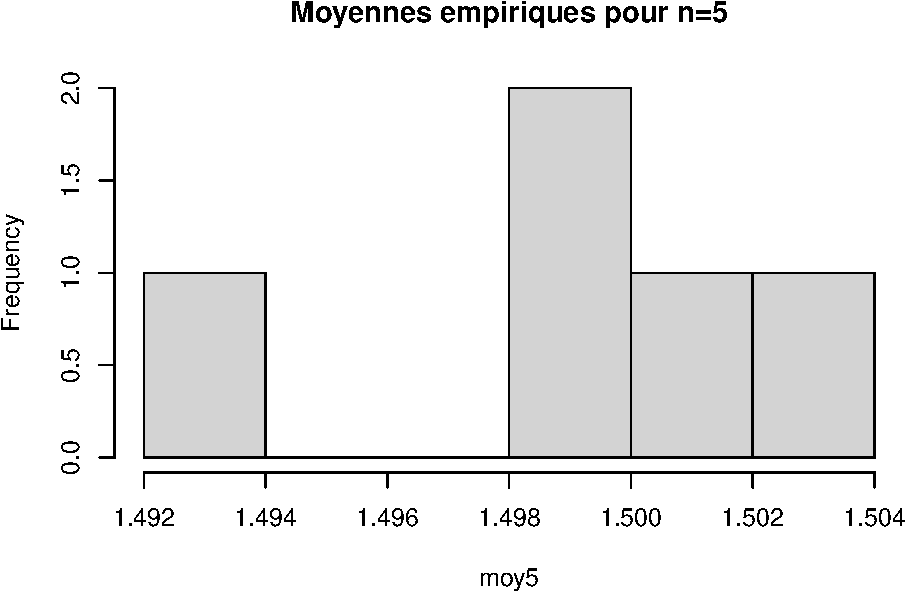
\includegraphics{tp2_files/figure-latex/echantillons-1.pdf}
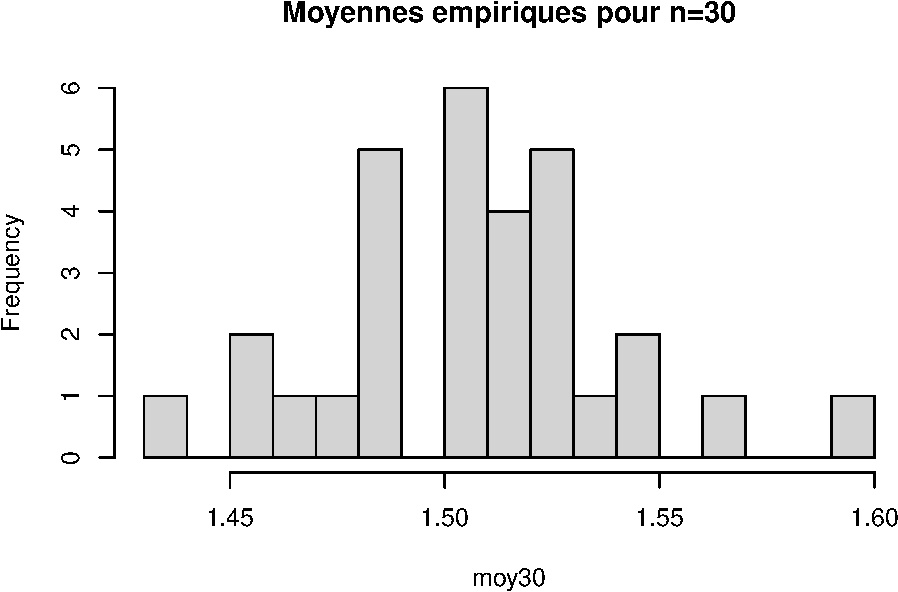
\includegraphics{tp2_files/figure-latex/echantillons-2.pdf}
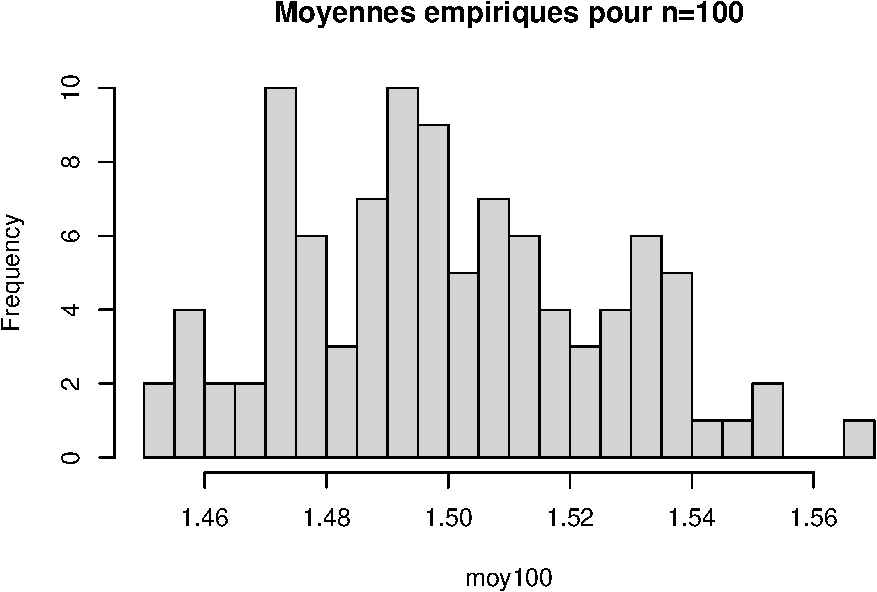
\includegraphics{tp2_files/figure-latex/echantillons-3.pdf}

\begin{enumerate}
\def\labelenumi{\arabic{enumi}.}
\setcounter{enumi}{3}
\tightlist
\item
  A l'aide d'une renormalisation adéquate (an, bn), montrer que Un,i =
  ¯Xn,i−an/ bn a une loi que vous pouvez approchez. Comparez histogramme
  de les moyennes empiriques normalisées, Un,i, et distribution
  théorique approchée. Quelle est l'influence de la taille de
  l'échantillon n sur la qualité de cette approximation?
\end{enumerate}

\begin{Shaded}
\begin{Highlighting}[]
\NormalTok{moy5CentreeReduite }\OtherTok{\textless{}{-}}\NormalTok{ (moy5}\SpecialCharTok{{-}}\FunctionTok{mean}\NormalTok{(moy5))}\SpecialCharTok{/}\FunctionTok{mean}\NormalTok{(moy5}\SpecialCharTok{\^{}}\DecValTok{2}\SpecialCharTok{/}\DecValTok{1000}\NormalTok{)}
\NormalTok{moy30CentreeReduite }\OtherTok{\textless{}{-}}\NormalTok{ (moy30}\SpecialCharTok{{-}}\FunctionTok{mean}\NormalTok{(moy30))}\SpecialCharTok{/}\FunctionTok{mean}\NormalTok{(moy30}\SpecialCharTok{\^{}}\DecValTok{2}\SpecialCharTok{/}\DecValTok{1000}\NormalTok{)}
\NormalTok{moy100CentreeReduite }\OtherTok{\textless{}{-}}\NormalTok{ (moy100}\SpecialCharTok{{-}}\FunctionTok{mean}\NormalTok{(moy100))}\SpecialCharTok{/}\FunctionTok{mean}\NormalTok{(moy100}\SpecialCharTok{\^{}}\DecValTok{2}\SpecialCharTok{/}\DecValTok{1000}\NormalTok{)}

\FunctionTok{hist}\NormalTok{(moy5CentreeReduite)}
\FunctionTok{lines}\NormalTok{(}\FunctionTok{seq}\NormalTok{(}\SpecialCharTok{{-}}\DecValTok{50}\NormalTok{,}\DecValTok{50}\NormalTok{,}\AttributeTok{by=}\FloatTok{0.1}\NormalTok{),}\FunctionTok{dpareto}\NormalTok{(}\FunctionTok{seq}\NormalTok{(}\SpecialCharTok{{-}}\DecValTok{50}\NormalTok{,}\DecValTok{50}\NormalTok{,}\AttributeTok{by=}\FloatTok{0.1}\NormalTok{),}\DecValTok{1}\NormalTok{,}\DecValTok{3}\NormalTok{),}\AttributeTok{col =} \StringTok{"blue"}\NormalTok{)}
\end{Highlighting}
\end{Shaded}

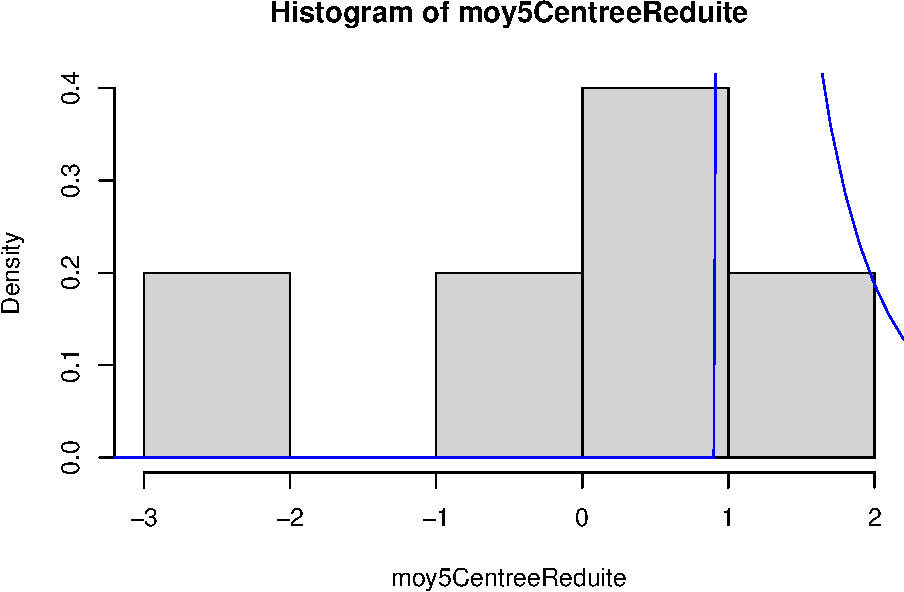
\includegraphics{tp2_files/figure-latex/normalisation-1.pdf}

\begin{Shaded}
\begin{Highlighting}[]
\FunctionTok{hist}\NormalTok{(moy30CentreeReduite,}\AttributeTok{breaks =} \DecValTok{10}\NormalTok{)}
\FunctionTok{lines}\NormalTok{(}\FunctionTok{seq}\NormalTok{(}\SpecialCharTok{{-}}\DecValTok{50}\NormalTok{,}\DecValTok{50}\NormalTok{,}\AttributeTok{by=}\FloatTok{0.1}\NormalTok{),}\FunctionTok{dpareto}\NormalTok{(}\FunctionTok{seq}\NormalTok{(}\SpecialCharTok{{-}}\DecValTok{50}\NormalTok{,}\DecValTok{50}\NormalTok{,}\AttributeTok{by=}\FloatTok{0.1}\NormalTok{),}\DecValTok{1}\NormalTok{,}\DecValTok{3}\NormalTok{),}\AttributeTok{col =} \StringTok{"blue"}\NormalTok{)}
\end{Highlighting}
\end{Shaded}

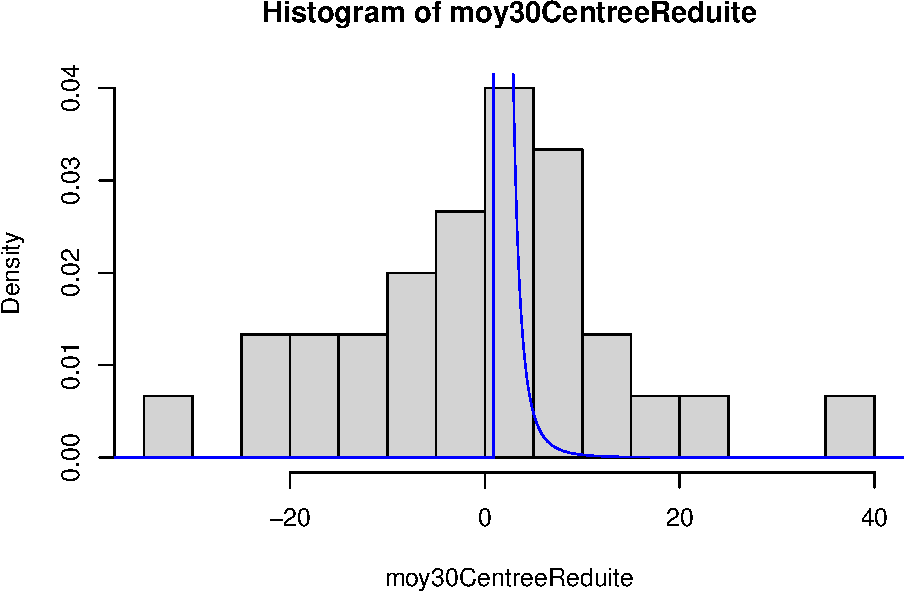
\includegraphics{tp2_files/figure-latex/normalisation-2.pdf}

\begin{Shaded}
\begin{Highlighting}[]
\FunctionTok{hist}\NormalTok{(moy100CentreeReduite,}\AttributeTok{breaks =} \DecValTok{20}\NormalTok{)}
\FunctionTok{lines}\NormalTok{(}\FunctionTok{seq}\NormalTok{(}\SpecialCharTok{{-}}\DecValTok{50}\NormalTok{,}\DecValTok{50}\NormalTok{,}\AttributeTok{by=}\FloatTok{0.1}\NormalTok{),}\FunctionTok{dpareto}\NormalTok{(}\FunctionTok{seq}\NormalTok{(}\SpecialCharTok{{-}}\DecValTok{50}\NormalTok{,}\DecValTok{50}\NormalTok{,}\AttributeTok{by=}\FloatTok{0.1}\NormalTok{),}\DecValTok{1}\NormalTok{,}\DecValTok{3}\NormalTok{),}\AttributeTok{col =} \StringTok{"blue"}\NormalTok{)}
\end{Highlighting}
\end{Shaded}

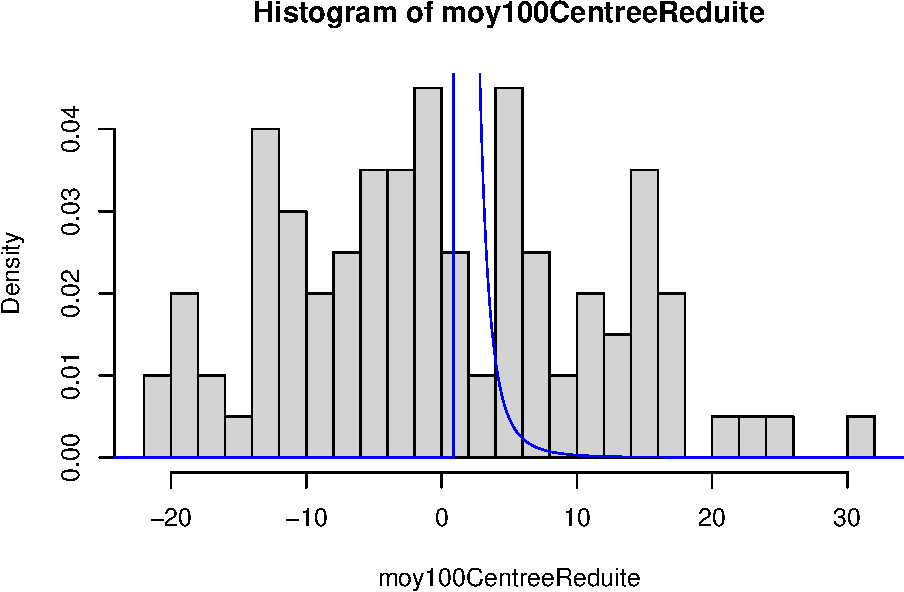
\includegraphics{tp2_files/figure-latex/normalisation-3.pdf}

\hypertarget{quand-le-thuxe9oruxe8me-de-central-limite-ne-sapplique-pas}{%
\subsection{Quand le théorème de central limite ne s'applique
pas}\label{quand-le-thuxe9oruxe8me-de-central-limite-ne-sapplique-pas}}

1. Simuler un échantillon de taille n = 20 d'une loi de C(2) et calculer
la moyenne empirique ¯Xn.

Moyenne empirique:

\begin{verbatim}
## [1] 1.516915
\end{verbatim}

2. Faites varier la taille de l'échantillon n = 20, 100, 1000 et 10000.
Qu'en déduire ?

\begin{verbatim}
## [1] 6.068616
\end{verbatim}

\begin{verbatim}
## [1] 1.684488
\end{verbatim}

\begin{verbatim}
## [1] 2.765645
\end{verbatim}

\begin{verbatim}
## [1] 1.222625
\end{verbatim}

\end{document}
